\documentclass{article} 

\usepackage[brazil]{babel}
\usepackage{enumitem}
\usepackage{amsmath}
\usepackage{booktabs}
\usepackage{bm}
\usepackage{float}
\usepackage[margin=2cm]{geometry}
\usepackage{circuitikz}
\usepackage{siunitx}
\usepackage{steinmetz}
\usepackage{amssymb}

\newcommand{\phasor}[2]{%
  #1 \, \phase{\, #2^\circ} \,
}

% \newcommand{\phasor}[2]{%
%   #1 \, \text{\phase{\, \ang{#2}}} \,
% }

\newcommand{\nle}{%
  \notag \\[4pt]
}

\setlength{\parindent}{0pt}

\title{Modelagem Matemática da Microrrede CC} 
\author{} 
% \date{\today}
\date{}

\begin{document}

\maketitle

\subsection*{Esquemático da Microrrede}

\begin{figure}[h]
  \centering
  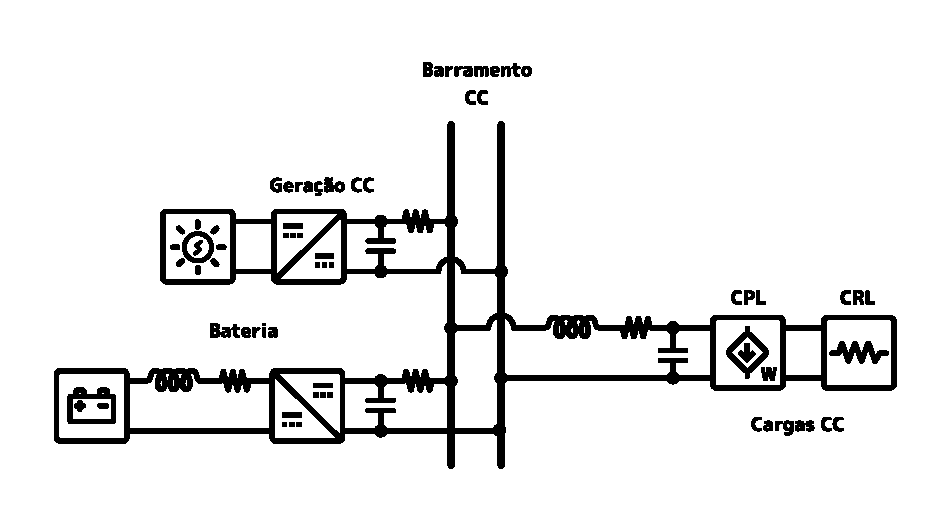
\includegraphics[scale=0.87]{assets/dc_microgrid.eps}
  \caption{Esquemático da Microrrede CC}
  \label{fig:exemplo}
\end{figure}

\subsubsection*{Modelagem do Subsistema: Geração CC}

O circuito da geração CC está representado abaixo:

\begin{figure}[H]
  \centering
  \begin{circuitikz}[american, scale=0.5, font=\footnotesize]
    \ctikzset{bipoles/length=1cm}
    \draw
      (0,4) to[vsource, v_=$v_G(t)$] (0,0)
      (0,4) to[normal open switch, l=$S_G$] (4,4)
      (4,0) to[diode, l=$D_G$] (4,4)
      (4,4) to[L, l=$L_G$, i_=$i_{L_G}(t)$] (8,4)
      (7,4) to[R, l=$R_{G_1}$] (11,4)
      (11,4) to[C, l=$C_G$, v=$v_{C_G}(t)$] (11,0)
      (11,4) to[R, l=$R_{G_2}$, i_=$i_{G}(t)$] (15,4)

      (15,4) to[short, -o] (16,4)
      (0,0) to[short, -o] (16,0)

      (16,4) to[open, v=$v_E(t)$] (16,0)
    ;
  \end{circuitikz}
\end{figure}

Aplicando a LKT na segunda malha a partir da esquerda, obtemos:
\begin{gather}
  d_G(t) v_G(t) - L_G \dot{i}_{L_G} - R_{G_1} i_{L_G}(t) - v_{C_G}(t) = 0 \nle
  \dot{i}_{L_G} = - \frac{R_{G_1}}{L_G} i_{L_G}(t) - \frac{1}{L_G} v_{C_G}(t) + \frac{v_G(t)}{L_G} d_G(t)
\end{gather}

Aplicando a LKC, obtemos:
\begin{gather}
  i_{L_G}(t) = C_G \dot{v}_{C_G} + i_G(t)
\end{gather}

Têm-se que, $i_G(t) = \frac{v_{C_G}(t) - v_E(t)}{R_{G_2}}$. Logo,
\begin{gather}
  i_{L_G}(t) = C_G \dot{v}_{C_G} + \frac{1}{R_{G_2}}v_{C_G}(t) - \frac{1}{R_{G_2}} v_E(t) \nle
  i_{L_G}(t) = C_G \dot{v}_{C_G} + \frac{1}{R_{G_2}}v_{C_G}(t) - \frac{1}{R_{G_2}} v_E(t) \nle
  \dot{v}_{C_G} = \frac{1}{C_G} i_{L_G}(t) - \frac{1}{R_{G_2}C_G }v_{C_G}(t) + \frac{1}{R_{G_2} C_G} v_E(t)
\end{gather}

Portanto, o modelo do subsistema da bateria é:

\begin{gather}
  \begin{cases}
    \dot{i}_{L_G} = \displaystyle - \frac{R_{G_1}}{L_G} i_{L_G}(t) - \frac{1}{L_G} v_{C_G}(t) + \frac{v_G(t)}{L_G} d_G(t) \\[12pt]
    \dot{v}_{C_G} = \displaystyle \frac{1}{C_G} i_{L_G}(t) - \frac{1}{R_{G_2}C_G }v_{C_G}(t) + \frac{1}{R_{G_2} C_G} v_E(t)
  \end{cases}
\end{gather}

\end{document}
